\subsection{Aves: complexidade de habitats e diversidade} % Rodolpho
\label{sec:compl-de-habit} 


Até o momento foram realizadas duas das três saídas de campo previstas para este subprojeto. Na primeira campanha, realizada entre 8 e 30 de maio, foram feitos o reconhecimento das áreas, demarcação dos pontos a serem amostrados e o teste dos métodos amostrais. No total, foram demarcados 32 pontos amostrais, distribuídos entre três fitofisionomias distintas de Cerrado, a saber: campo sujo, campo cerrado e cerrado \textit{sensu stricto}. Estas fitofisionomias foram escolhidas por representarem um gradiente de estrutura vegetacional, que aumenta do campo sujo para o cerrado \textit{sensu stricto}, sendo o campo cerrado a forma intermediária. Cada um dos pontos amostrais consiste de dois transectos de 200 m. Também nesta primeira campanha foram testados dois métodos amostrais para o levantamento da diversidade de aves: método de ponto fixo e método de transecto. Ambos os métodos se baseiam no registro visual e auditivo das espécies de aves durante certo intervalo de tempo, porém o método de ponto fixo consiste no registro das espécies pelo observador enquanto este se encontra parado em um determinado ponto. No método de transecto, o observador se locomove por um trajeto (em velocidade constante) enquanto registra as espécies que visualiza/escuta.
Durante esta primeira campanha foram realizados 586 registros de 94 espécies, sendo que dentre estes alguns merecem destaque. A espécie \textit{Urubitinga coronata} (Águia-cinzenta) consta na categoria "Em perigo" da lista nacional de espécies em extinção (MMA, Portaria nº444 de 17 de dezembro 2014) e também na lista de espécies de extinção de Minas Gerais (DN COPAM nº147, de 30 de abril de 2010). Outras espécies que constam na lista de espécies ameaçadas de Minas Gerais são: \textit{Mycteria americana} (Cabeça-seca, categoria "Vulnerável"), \textit{Crax fasciolata} (Mutum-de-penacho,categoria "Em perigo"), \textit{Sporophila angolensis} (Curió, categoria "Criticamente em Perigo"), \textit{Ara ararauna}  (Arara-canindé, categoria "Vulnerável"), \textit{Ara chloropterus} (Arara-vermelha-grande, categoria "Criticamente em Perigo").
Considerando os dois diferntes métodos amostrais empregados nesta primeira campanha, 331 registros de 60 espécies foram realizados usando o método de ponto de escuta e 225 registros de 65 espécies foram feitos utilizando o método de transecto.
A proposta inicial do projeto era utilizar o método de ponto de escuta, pois um dos objetivos do projeto (quantificação do uso dos estratos vegetais pelas aves) depende da visualização dos indivíduos, e nós acreditávamos que esta visualização poderia ser facilitada se o observador estivesse parado em um mesmo local. No entanto, o método de ponto fixo apresentou um baixo percentual do total de registros na forma de contatos visuais (apenas 18\% de todos os contatos), enquanto que o método de transecto se mostrou mais efetivo para a observação e registro visual das aves (48\% de todos os registros)(Figura \ref{fig:Figura 1}). Assim, este resultado nos motivou a escolher pelo método de transecto para a continuidade do trabalho.

\begin{figure}[hbtp]
\centering
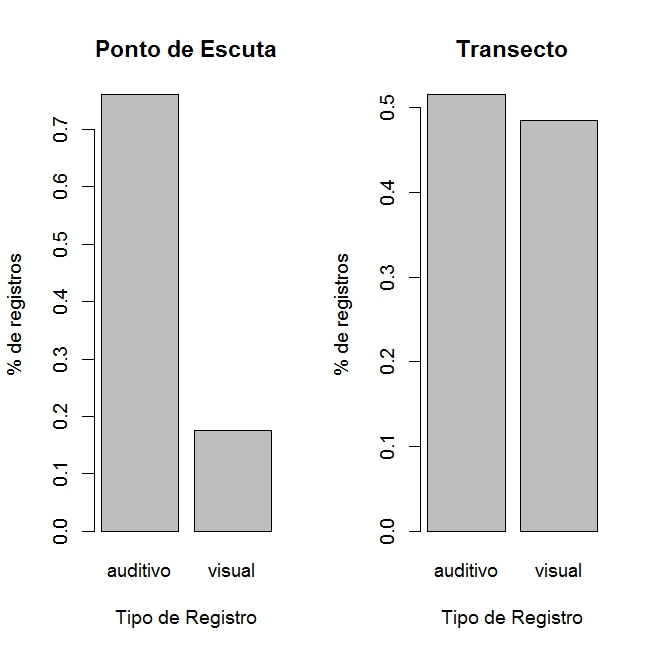
\includegraphics[scale=0.55]{dados_piloto.jpg}
\caption{Proporção de registros auditivos e visuais realizados a partir dos métodos de ponto de escuta e transecto, respectivamente. Note que o comprimento do eixo y é diferente entre os dois gráficos.}

\label{fig:Figura 1} 
\end{figure}


Na segunda campanha, realizada entre 25 de novembro e 17 dezembro de 2014, foi realizada a primeira etapa das amostragens nos 32 pontos amostrais selecionados previamente. Durante esta campanha foram contabilizados 1925 registros de aves de 141 espécies, sendo que dentre estas foi registrada a espécie \textit{Tigrisoma fasciatum} (Socó-boi-escuro),considerada como "Vulnerável" em nível nacional (MMA, Portaria nº444 de 17 de dezembro 2014) e "Criticamente em Perigo" em Minas Gerais. Outras espécies que constam na lista de espécies ameaçadas de Minas Gerais e foram registradas neste período foram: Culicivora caudacuta(Papa-moscas-do-campo, categoria "Vulnerável"), Euscarthmus rufomarginatus (Maria-corruíra, categoria "Criticamente em Perigo"), Suiriri islerorum (Suiriri-da-chapada, categoria "Vulnerável"), além de \textit{M. americana}, \textit{S. angolensis} e \textit{A. ararauna}, já registradas durante a primeira campanha.

As amostragens foram realizadas nos períodos da manhã (entre 06:00 e 11:00) e à tarde (entre 15:30 e 20:00) e cada registro foi  individualizado considerando a presença da ave dentro ou fora da região amostral (dentro ou fora de raio de 100m em torno do ponto) e o tipo de registro (visual ou auditivo). Nos registros visuais, foram também registrados a distância perpendicular das aves em relação ao transecto, a qual será utilizada para avaliar o efeito da distância de observação na detecção das espécies, e também o estrato vegetacional que o indivíduo foi avistado, a qual será usada em uma etapa posterior para avaliação do efeito da complexidade de habitats sobre a diversidade de espécies.
Com relação às três fitofisionomias amostradas, o maior número de registros foi realizado na fitofisionomia campo cerrado (653), seguido por campo sujo (640) e cerrado \textit{sensu stricto} (625). Entretanto, quando consideramos o número de registros realizados dentro ou fora do raio amostral de 100 m em torno dos pontos amostrais, os resultados são qualitativamente diferentes.
Os registros dentro do raio amostral de 100m foram maiores na fitofisionomia campo sujo (334), depois em campo cerrado (269) e por último em cerrado \textit{sensu stricto} (Figura \ref{fig:Figura 2}). Já para os registros realizados fora do raio de 100 m torno dos pontos amostrais, a fitofisionomia que apresentou maior número de registros foi o cerrado \textit{sensu stricto} (414), depois o campo cerrado (384) e por último o campo sujo (306) (Figura \ref{fig:Figura 2}).

\begin{figure}[hbtp]
\centering
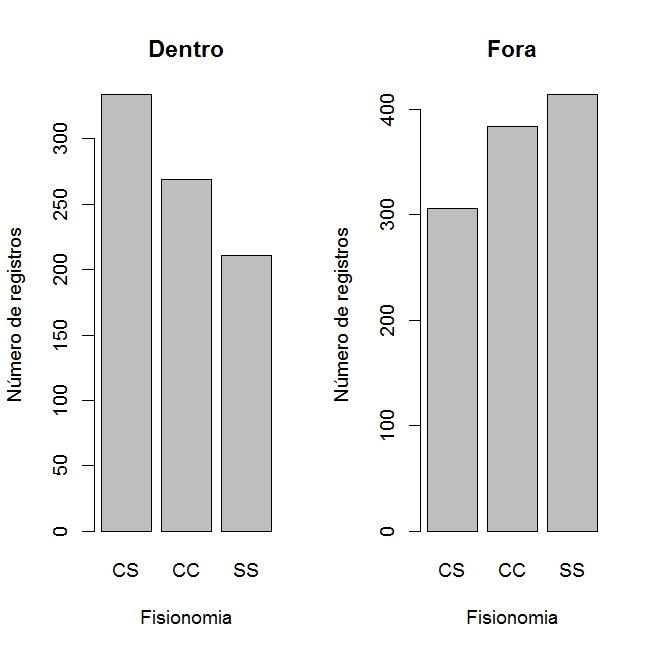
\includegraphics[scale=0.55]{reg_fito.jpg}
\caption{Número de registros de aves realizados em cada uma das fitofisionomias amostradas, considerando os rgistros feitos dentro do raio amostral de 100m e fora deste raio amostral. Legenda: CS- Campo sujo; CC -  Campo Cerrado; SS- Cerrado \textit{Sensu stricto}. Note que o comprimento do eixo y é diferente entre os dois gráficos.}

\label{fig:Figura 2} 
\end{figure}


O maior número de espécies dentro das áreas amostrais foi registrado na fitofisionomia campo cerrado (67), seguido por cerrado \textit{sensu stricto} (64) e campo sujo (60) (Figura \ref{fig:Figura 3}). Entretanto, quando consideramos o número de espécies registrado fora da áreas amostrais, a fitofisionomia campo sujo apresentou um maior número de espécies (63), seguido por campo cerrado (59) e cerrado \textit{sensu stricto}(26)(Figura \ref{fig:Figura 3}).


\begin{figure}[hbtp]
\centering
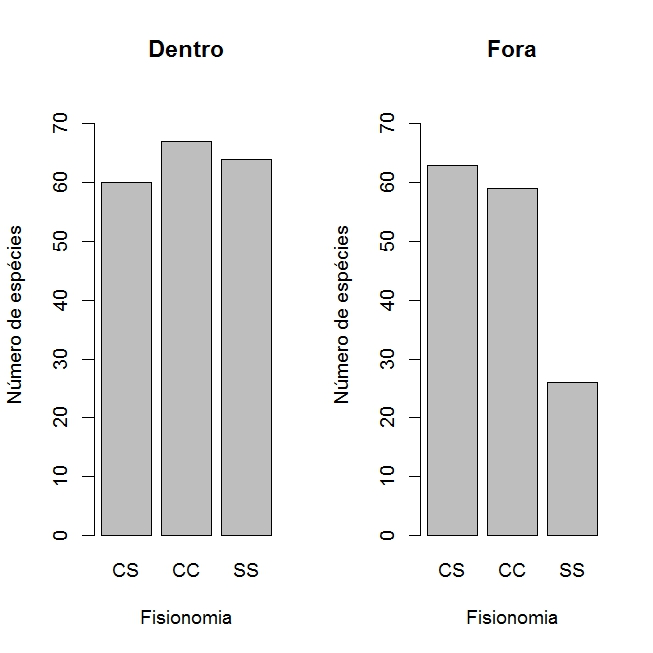
\includegraphics[scale=0.55]{dados_fito.jpg}
\caption{Número de espécies registradas em cada uma das fitofisionomias amostradas, considerando os rgistros feitos dentro do raio amostral de 100m e fora deste raio amostral. Legenda: CS- Campo sujo; CC -  Campo Cerrado; SS- Cerrado \textit{Sensu stricto}. Note que o comprimento do eixo y é diferente entre os dois gráficos.}

\label{fig:Figura 3} 
\end{figure}

Estes resultados preliminares indicam que o número de registros feitos em cada fitofisionomia, assim como o número de espécies presentes em cada uma, são diferentes. Além disso, estes resultados indicam que existe um efeito da distância que os registros foram realizados, já que os registros e espécies encontrados dentro e fora do raio de 100m em torno dos pontos apresentam diferentes padrões. Este efeito da distância pode ocorrer tanto por uma maior heterogeneidade de hábitats em torno de algumas fitofisionomias em relação à outras quanto por um efeito da detectabilidade associado às características dos hábitats, já que o efeito positivo da vegetação sobre o número de espécies poderia ser reduzido ou até mascarado por um efeito negativo da vegetação sobre a detecção das espécies. Ao final da coleta e das análises dos dados, esperamos obter uma maior compreensão sobre a influência da complexidade dos habitats sobre a diversidade de aves, assim como também um melhor entendimento dos fatores que podem influenciar a detecção destes padrões.